\documentclass[twoside]{book}

% Packages required by doxygen
\usepackage{calc}
\usepackage{doxygen}
\usepackage{graphicx}
\usepackage[utf8]{inputenc}
\usepackage{makeidx}
\usepackage{multicol}
\usepackage{multirow}
\usepackage{fixltx2e}
\PassOptionsToPackage{warn}{textcomp}
\usepackage{textcomp}
\usepackage[nointegrals]{wasysym}
\usepackage[table]{xcolor}

% Font selection
\usepackage[T1]{fontenc}
\usepackage{mathptmx}
\usepackage[scaled=.90]{helvet}
\usepackage{courier}
\usepackage{amssymb}
\usepackage{sectsty}
\renewcommand{\familydefault}{\sfdefault}
\allsectionsfont{%
  \fontseries{bc}\selectfont%
  \color{darkgray}%
}
\renewcommand{\DoxyLabelFont}{%
  \fontseries{bc}\selectfont%
  \color{darkgray}%
}
\newcommand{\+}{\discretionary{\mbox{\scriptsize$\hookleftarrow$}}{}{}}

% Page & text layout
\usepackage{geometry}
\geometry{%
  a4paper,%
  top=2.5cm,%
  bottom=2.5cm,%
  left=2.5cm,%
  right=2.5cm%
}
\tolerance=750
\hfuzz=15pt
\hbadness=750
\setlength{\emergencystretch}{15pt}
\setlength{\parindent}{0cm}
\setlength{\parskip}{0.2cm}
\makeatletter
\renewcommand{\paragraph}{%
  \@startsection{paragraph}{4}{0ex}{-1.0ex}{1.0ex}{%
    \normalfont\normalsize\bfseries\SS@parafont%
  }%
}
\renewcommand{\subparagraph}{%
  \@startsection{subparagraph}{5}{0ex}{-1.0ex}{1.0ex}{%
    \normalfont\normalsize\bfseries\SS@subparafont%
  }%
}
\makeatother

% Headers & footers
\usepackage{fancyhdr}
\pagestyle{fancyplain}
\fancyhead[LE]{\fancyplain{}{\bfseries\thepage}}
\fancyhead[CE]{\fancyplain{}{}}
\fancyhead[RE]{\fancyplain{}{\bfseries\leftmark}}
\fancyhead[LO]{\fancyplain{}{\bfseries\rightmark}}
\fancyhead[CO]{\fancyplain{}{}}
\fancyhead[RO]{\fancyplain{}{\bfseries\thepage}}
\fancyfoot[LE]{\fancyplain{}{}}
\fancyfoot[CE]{\fancyplain{}{}}
\fancyfoot[RE]{\fancyplain{}{\bfseries\scriptsize Generated on Tue Aug 4 2015 11\+:33\+:36 for Blendshade by Doxygen }}
\fancyfoot[LO]{\fancyplain{}{\bfseries\scriptsize Generated on Tue Aug 4 2015 11\+:33\+:36 for Blendshade by Doxygen }}
\fancyfoot[CO]{\fancyplain{}{}}
\fancyfoot[RO]{\fancyplain{}{}}
\renewcommand{\footrulewidth}{0.4pt}
\renewcommand{\chaptermark}[1]{%
  \markboth{#1}{}%
}
\renewcommand{\sectionmark}[1]{%
  \markright{\thesection\ #1}%
}

% Indices & bibliography
\usepackage{natbib}
\usepackage[titles]{tocloft}
\setcounter{tocdepth}{3}
\setcounter{secnumdepth}{5}
\makeindex

% Hyperlinks (required, but should be loaded last)
\usepackage{ifpdf}
\ifpdf
  \usepackage[pdftex,pagebackref=true]{hyperref}
\else
  \usepackage[ps2pdf,pagebackref=true]{hyperref}
\fi
\hypersetup{%
  colorlinks=true,%
  linkcolor=blue,%
  citecolor=blue,%
  unicode%
}

% Custom commands
\newcommand{\clearemptydoublepage}{%
  \newpage{\pagestyle{empty}\cleardoublepage}%
}


%===== C O N T E N T S =====

\begin{document}

% Titlepage & ToC
\hypersetup{pageanchor=false,
             bookmarks=true,
             bookmarksnumbered=true,
             pdfencoding=unicode
            }
\pagenumbering{roman}
\begin{titlepage}
\vspace*{7cm}
\begin{center}%
{\Large Blendshade \\[1ex]\large 1.\+0 }\\
\vspace*{1cm}
{\large Generated by Doxygen 1.8.7}\\
\vspace*{0.5cm}
{\small Tue Aug 4 2015 11:33:36}\\
\end{center}
\end{titlepage}
\clearemptydoublepage
\tableofcontents
\clearemptydoublepage
\pagenumbering{arabic}
\hypersetup{pageanchor=true}

%--- Begin generated contents ---
\chapter{Hierarchical Index}
\section{Class Hierarchy}
This inheritance list is sorted roughly, but not completely, alphabetically\+:\begin{DoxyCompactList}
\item \contentsline{section}{I\+Laplacian\+Data}{\pageref{class_i_laplacian_data}}{}
\begin{DoxyCompactList}
\item \contentsline{section}{Mesh\+Laplacian\+Data}{\pageref{class_mesh_laplacian_data}}{}
\end{DoxyCompactList}
\item \contentsline{section}{Maya\+Eigen}{\pageref{class_maya_eigen}}{}
\item M\+Px\+Deformer\+Node\begin{DoxyCompactList}
\item \contentsline{section}{Laplacian\+Smoother}{\pageref{class_laplacian_smoother}}{}
\end{DoxyCompactList}
\item \contentsline{section}{Time\+Counter}{\pageref{class_time_counter}}{}
\end{DoxyCompactList}

\chapter{Class Index}
\section{Class List}
Here are the classes, structs, unions and interfaces with brief descriptions\+:\begin{DoxyCompactList}
\item\contentsline{section}{\hyperlink{class_i_laplacian_data}{I\+Laplacian\+Data} \\*Interface class for Laplacian data }{\pageref{class_i_laplacian_data}}{}
\item\contentsline{section}{\hyperlink{class_laplacian_smoother}{Laplacian\+Smoother} \\*\hyperlink{class_laplacian_smoother}{Laplacian\+Smoother} implementation }{\pageref{class_laplacian_smoother}}{}
\item\contentsline{section}{\hyperlink{class_maya_eigen}{Maya\+Eigen} \\*\hyperlink{class_maya_eigen}{Maya\+Eigen} implementation }{\pageref{class_maya_eigen}}{}
\item\contentsline{section}{\hyperlink{class_mesh_laplacian_data}{Mesh\+Laplacian\+Data} \\*Laplacian data }{\pageref{class_mesh_laplacian_data}}{}
\item\contentsline{section}{\hyperlink{class_time_counter}{Time\+Counter} \\*\hyperlink{class_time_counter}{Time\+Counter} implementation }{\pageref{class_time_counter}}{}
\end{DoxyCompactList}

\chapter{File Index}
\section{File List}
Here is a list of all documented files with brief descriptions\+:\begin{DoxyCompactList}
\item\contentsline{section}{C\+:/\+Users/tody/\+Documents/\+Git\+Hub/\+Maya\+Plugin\+Samples/\+Laplacian\+Smoother/src/{\bfseries I\+Laplacian\+Data.\+h} }{\pageref{_i_laplacian_data_8h}}{}
\item\contentsline{section}{C\+:/\+Users/tody/\+Documents/\+Git\+Hub/\+Maya\+Plugin\+Samples/\+Laplacian\+Smoother/src/\hyperlink{_init_plugin_8cpp}{Init\+Plugin.\+cpp} \\*Plugin functions for \hyperlink{class_laplacian_smoother}{Laplacian\+Smoother} }{\pageref{_init_plugin_8cpp}}{}
\item\contentsline{section}{C\+:/\+Users/tody/\+Documents/\+Git\+Hub/\+Maya\+Plugin\+Samples/\+Laplacian\+Smoother/src/\hyperlink{_laplacian_smoother_8cpp}{Laplacian\+Smoother.\+cpp} \\*\hyperlink{class_laplacian_smoother}{Laplacian\+Smoother} definition }{\pageref{_laplacian_smoother_8cpp}}{}
\item\contentsline{section}{C\+:/\+Users/tody/\+Documents/\+Git\+Hub/\+Maya\+Plugin\+Samples/\+Laplacian\+Smoother/src/\hyperlink{_laplacian_smoother_8h}{Laplacian\+Smoother.\+h} }{\pageref{_laplacian_smoother_8h}}{}
\item\contentsline{section}{C\+:/\+Users/tody/\+Documents/\+Git\+Hub/\+Maya\+Plugin\+Samples/\+Laplacian\+Smoother/src/\hyperlink{_maya_eigen_8cpp}{Maya\+Eigen.\+cpp} \\*\hyperlink{class_laplacian_smoother}{Laplacian\+Smoother} definition }{\pageref{_maya_eigen_8cpp}}{}
\item\contentsline{section}{C\+:/\+Users/tody/\+Documents/\+Git\+Hub/\+Maya\+Plugin\+Samples/\+Laplacian\+Smoother/src/\hyperlink{_maya_eigen_8h}{Maya\+Eigen.\+h} }{\pageref{_maya_eigen_8h}}{}
\item\contentsline{section}{C\+:/\+Users/tody/\+Documents/\+Git\+Hub/\+Maya\+Plugin\+Samples/\+Laplacian\+Smoother/src/{\bfseries Mesh\+Laplacian\+Data.\+h} }{\pageref{_mesh_laplacian_data_8h}}{}
\item\contentsline{section}{C\+:/\+Users/tody/\+Documents/\+Git\+Hub/\+Maya\+Plugin\+Samples/\+Laplacian\+Smoother/src/\hyperlink{_time_counter_8h}{Time\+Counter.\+h} \\*\hyperlink{class_time_counter}{Time\+Counter} class definition }{\pageref{_time_counter_8h}}{}
\end{DoxyCompactList}

\chapter{Class Documentation}
\hypertarget{class_i_laplacian_data}{\section{I\+Laplacian\+Data Class Reference}
\label{class_i_laplacian_data}\index{I\+Laplacian\+Data@{I\+Laplacian\+Data}}
}


Interface class for Laplacian data.  




{\ttfamily \#include $<$I\+Laplacian\+Data.\+h$>$}

Inheritance diagram for I\+Laplacian\+Data\+:\begin{figure}[H]
\begin{center}
\leavevmode
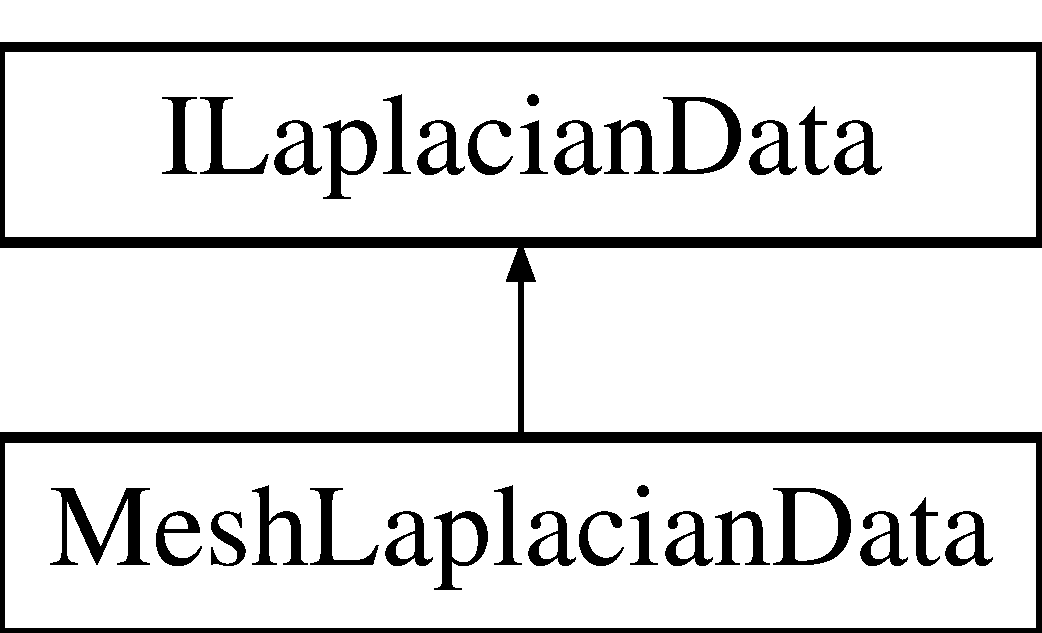
\includegraphics[height=2.000000cm]{class_i_laplacian_data}
\end{center}
\end{figure}
\subsection*{Public Member Functions}
\begin{DoxyCompactItemize}
\item 
\hyperlink{class_i_laplacian_data_a71e44bc645284129993f1563e199df2d}{I\+Laplacian\+Data} (const M\+Dag\+Path \&geometry\+Path)
\item 
\hyperlink{class_i_laplacian_data_a34b9877ebb8024d518dd0c47e48f99fa}{I\+Laplacian\+Data} (const M\+Object \&geometry\+Object)
\item 
\hypertarget{class_i_laplacian_data_a2664db9f1fefe4cbc8415ef9f90bfe60}{virtual \hyperlink{class_i_laplacian_data_a2664db9f1fefe4cbc8415ef9f90bfe60}{$\sim$\+I\+Laplacian\+Data} ()}\label{class_i_laplacian_data_a2664db9f1fefe4cbc8415ef9f90bfe60}

\begin{DoxyCompactList}\small\item\em Destructor. \end{DoxyCompactList}\item 
virtual const \\*
Eigen\+::\+Sparse\+Matrix$<$ double $>$ \hyperlink{class_i_laplacian_data_ae5d1999d7e077fae5e415ce811d71dba}{Get\+Laplacian\+Matrix} (int num\+Functions=3)=0
\begin{DoxyCompactList}\small\item\em Get Laplacian data. \end{DoxyCompactList}\end{DoxyCompactItemize}
\subsection*{Protected Attributes}
\begin{DoxyCompactItemize}
\item 
\hypertarget{class_i_laplacian_data_a9e9b48a29dff036d051ed7aa82aa0e88}{M\+Object \hyperlink{class_i_laplacian_data_a9e9b48a29dff036d051ed7aa82aa0e88}{\+\_\+geometry\+Object}}\label{class_i_laplacian_data_a9e9b48a29dff036d051ed7aa82aa0e88}

\begin{DoxyCompactList}\small\item\em Target geometry objet. \end{DoxyCompactList}\item 
\hypertarget{class_i_laplacian_data_addd290ef0f5373d84197af5d357cc52c}{M\+Dag\+Path \hyperlink{class_i_laplacian_data_addd290ef0f5373d84197af5d357cc52c}{\+\_\+geometry\+Path}}\label{class_i_laplacian_data_addd290ef0f5373d84197af5d357cc52c}

\begin{DoxyCompactList}\small\item\em Target geometry dag path. \end{DoxyCompactList}\end{DoxyCompactItemize}


\subsection{Detailed Description}
Interface class for Laplacian data. 

\subsection{Constructor \& Destructor Documentation}
\hypertarget{class_i_laplacian_data_a71e44bc645284129993f1563e199df2d}{\index{I\+Laplacian\+Data@{I\+Laplacian\+Data}!I\+Laplacian\+Data@{I\+Laplacian\+Data}}
\index{I\+Laplacian\+Data@{I\+Laplacian\+Data}!I\+Laplacian\+Data@{I\+Laplacian\+Data}}
\subsubsection[{I\+Laplacian\+Data}]{\setlength{\rightskip}{0pt plus 5cm}I\+Laplacian\+Data\+::\+I\+Laplacian\+Data (
\begin{DoxyParamCaption}
\item[{const M\+Dag\+Path \&}]{geometry\+Path}
\end{DoxyParamCaption}
)}}\label{class_i_laplacian_data_a71e44bc645284129993f1563e199df2d}

\begin{DoxyParams}{Parameters}
{\em geometry\+Path} & target geometry dag path \\
\hline
\end{DoxyParams}
\hypertarget{class_i_laplacian_data_a34b9877ebb8024d518dd0c47e48f99fa}{\index{I\+Laplacian\+Data@{I\+Laplacian\+Data}!I\+Laplacian\+Data@{I\+Laplacian\+Data}}
\index{I\+Laplacian\+Data@{I\+Laplacian\+Data}!I\+Laplacian\+Data@{I\+Laplacian\+Data}}
\subsubsection[{I\+Laplacian\+Data}]{\setlength{\rightskip}{0pt plus 5cm}I\+Laplacian\+Data\+::\+I\+Laplacian\+Data (
\begin{DoxyParamCaption}
\item[{const M\+Object \&}]{geometry\+Object}
\end{DoxyParamCaption}
)}}\label{class_i_laplacian_data_a34b9877ebb8024d518dd0c47e48f99fa}

\begin{DoxyParams}{Parameters}
{\em geometry\+Object} & target geometry object \\
\hline
\end{DoxyParams}


\subsection{Member Function Documentation}
\hypertarget{class_i_laplacian_data_ae5d1999d7e077fae5e415ce811d71dba}{\index{I\+Laplacian\+Data@{I\+Laplacian\+Data}!Get\+Laplacian\+Matrix@{Get\+Laplacian\+Matrix}}
\index{Get\+Laplacian\+Matrix@{Get\+Laplacian\+Matrix}!I\+Laplacian\+Data@{I\+Laplacian\+Data}}
\subsubsection[{Get\+Laplacian\+Matrix}]{\setlength{\rightskip}{0pt plus 5cm}virtual const Eigen\+::\+Sparse\+Matrix$<$double$>$ I\+Laplacian\+Data\+::\+Get\+Laplacian\+Matrix (
\begin{DoxyParamCaption}
\item[{int}]{num\+Functions = {\ttfamily 3}}
\end{DoxyParamCaption}
)\hspace{0.3cm}{\ttfamily [pure virtual]}}}\label{class_i_laplacian_data_ae5d1999d7e077fae5e415ce811d71dba}


Get Laplacian data. 


\begin{DoxyParams}{Parameters}
{\em num\+Functions} & the number of functions (e.\+g. 3 for point xyz.) \\
\hline
\end{DoxyParams}
\begin{DoxyReturn}{Returns}
Laplacian\+Matrix output Laplacian matrix data. Eigen\+::\+Sparse\+Matrix$<$double$>$ type. 
\end{DoxyReturn}


Implemented in \hyperlink{class_mesh_laplacian_data_a9efe80838593c46fac7baa77ef506559}{Mesh\+Laplacian\+Data}.



The documentation for this class was generated from the following file\+:\begin{DoxyCompactItemize}
\item 
C\+:/\+Users/tody/\+Documents/\+Git\+Hub/\+Maya\+Plugin\+Samples/\+Laplacian\+Smoother/src/I\+Laplacian\+Data.\+h\end{DoxyCompactItemize}

\hypertarget{class_laplacian_smoother}{\section{Laplacian\+Smoother Class Reference}
\label{class_laplacian_smoother}\index{Laplacian\+Smoother@{Laplacian\+Smoother}}
}


\hyperlink{class_laplacian_smoother}{Laplacian\+Smoother} implementation.  




{\ttfamily \#include $<$Laplacian\+Smoother.\+h$>$}

Inheritance diagram for Laplacian\+Smoother\+:\begin{figure}[H]
\begin{center}
\leavevmode
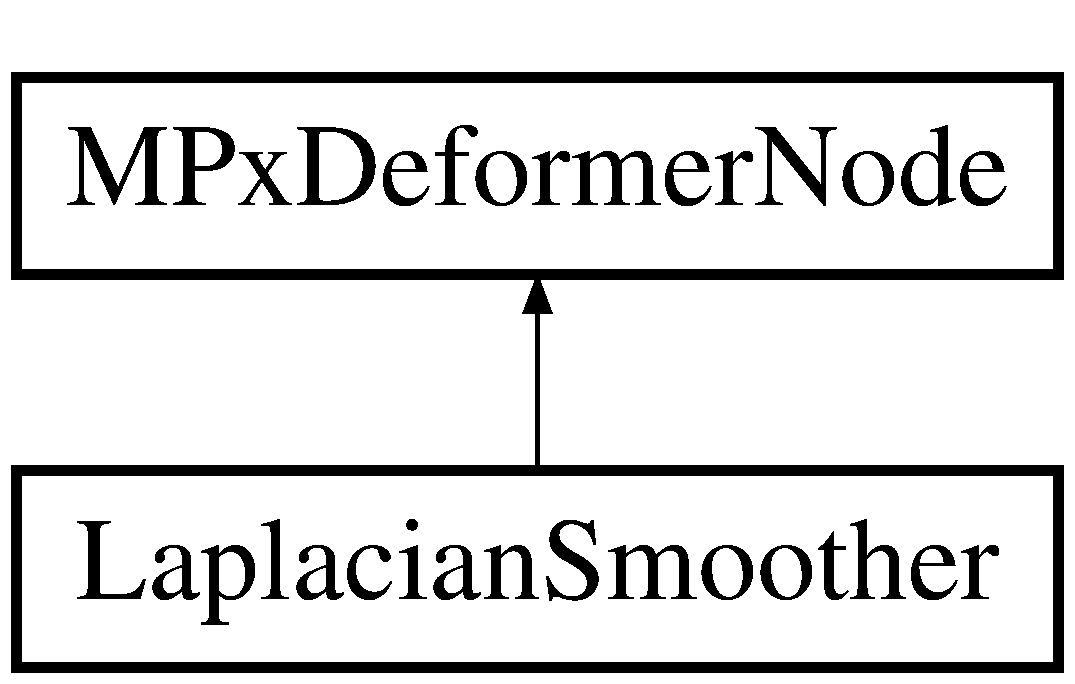
\includegraphics[height=2.000000cm]{class_laplacian_smoother}
\end{center}
\end{figure}
\subsection*{Public Member Functions}
\begin{DoxyCompactItemize}
\item 
\hypertarget{class_laplacian_smoother_abf02c86745e5c99a043ec0ac4974e5d5}{\hyperlink{class_laplacian_smoother_abf02c86745e5c99a043ec0ac4974e5d5}{Laplacian\+Smoother} ()}\label{class_laplacian_smoother_abf02c86745e5c99a043ec0ac4974e5d5}

\begin{DoxyCompactList}\small\item\em Constructor. \end{DoxyCompactList}\item 
\hypertarget{class_laplacian_smoother_ac7c1d554540a1168f7e2d76e003dadfb}{virtual \hyperlink{class_laplacian_smoother_ac7c1d554540a1168f7e2d76e003dadfb}{$\sim$\+Laplacian\+Smoother} ()}\label{class_laplacian_smoother_ac7c1d554540a1168f7e2d76e003dadfb}

\begin{DoxyCompactList}\small\item\em Destructor. \end{DoxyCompactList}\item 
M\+Status \hyperlink{class_laplacian_smoother_aa7c21d1acfef33eefbd020c959fa1eb0}{compute} (const M\+Plug \&plug, M\+Data\+Block \&data\+Block)
\begin{DoxyCompactList}\small\item\em Compute function to deform. \end{DoxyCompactList}\end{DoxyCompactItemize}
\subsection*{Static Public Member Functions}
\begin{DoxyCompactItemize}
\item 
static void $\ast$ \hyperlink{class_laplacian_smoother_a4775db7de0fe100ce7424b075cc88dcb}{creator} ()
\begin{DoxyCompactList}\small\item\em Create a new \hyperlink{class_laplacian_smoother}{Laplacian\+Smoother} instance. \end{DoxyCompactList}\item 
\hypertarget{class_laplacian_smoother_a6c5627afc523a4b436b167996db932ad}{static M\+Status \hyperlink{class_laplacian_smoother_a6c5627afc523a4b436b167996db932ad}{initialize} ()}\label{class_laplacian_smoother_a6c5627afc523a4b436b167996db932ad}

\begin{DoxyCompactList}\small\item\em Initializes the node attributes. \end{DoxyCompactList}\item 
\hypertarget{class_laplacian_smoother_a25f65e19e2b3953b850e2b246a7ff072}{static M\+String \hyperlink{class_laplacian_smoother_a25f65e19e2b3953b850e2b246a7ff072}{get\+Maya\+Name} ()}\label{class_laplacian_smoother_a25f65e19e2b3953b850e2b246a7ff072}

\begin{DoxyCompactList}\small\item\em Returns the type name of this node. \end{DoxyCompactList}\end{DoxyCompactItemize}
\subsection*{Static Public Attributes}
\begin{DoxyCompactItemize}
\item 
\hypertarget{class_laplacian_smoother_ab0803d4ade46ef489b64beb6114eb584}{static M\+Type\+Id \hyperlink{class_laplacian_smoother_ab0803d4ade46ef489b64beb6114eb584}{id}}\label{class_laplacian_smoother_ab0803d4ade46ef489b64beb6114eb584}

\begin{DoxyCompactList}\small\item\em type I\+D of the node. \end{DoxyCompactList}\end{DoxyCompactItemize}


\subsection{Detailed Description}
\hyperlink{class_laplacian_smoother}{Laplacian\+Smoother} implementation. 

argmin\+\_\+\+S $\vert$\+P -\/ S$\vert$$^\wedge$2 +  $\vert$ L S $\vert$$^\wedge$2

M = Lt L S = (I +  M)$^\wedge$\{-\/1\} P

M\+E\+L\+: deformer -\/type \hyperlink{class_laplacian_smoother}{Laplacian\+Smoother}; Python\+: cmds.\+deformer( type=\char`\"{}\+Laplacian\+Smoother\char`\"{} ); 

\subsection{Member Function Documentation}
\hypertarget{class_laplacian_smoother_aa7c21d1acfef33eefbd020c959fa1eb0}{\index{Laplacian\+Smoother@{Laplacian\+Smoother}!compute@{compute}}
\index{compute@{compute}!Laplacian\+Smoother@{Laplacian\+Smoother}}
\subsubsection[{compute}]{\setlength{\rightskip}{0pt plus 5cm}M\+Status Laplacian\+Smoother\+::compute (
\begin{DoxyParamCaption}
\item[{const M\+Plug \&}]{plug, }
\item[{M\+Data\+Block \&}]{data\+Block}
\end{DoxyParamCaption}
)}}\label{class_laplacian_smoother_aa7c21d1acfef33eefbd020c959fa1eb0}


Compute function to deform. 

If you want to access mesh structure from the deformer, you need to implement compute function replacing with deform function. \hypertarget{class_laplacian_smoother_a4775db7de0fe100ce7424b075cc88dcb}{\index{Laplacian\+Smoother@{Laplacian\+Smoother}!creator@{creator}}
\index{creator@{creator}!Laplacian\+Smoother@{Laplacian\+Smoother}}
\subsubsection[{creator}]{\setlength{\rightskip}{0pt plus 5cm}void $\ast$ Laplacian\+Smoother\+::creator (
\begin{DoxyParamCaption}
{}
\end{DoxyParamCaption}
)\hspace{0.3cm}{\ttfamily [static]}}}\label{class_laplacian_smoother_a4775db7de0fe100ce7424b075cc88dcb}


Create a new \hyperlink{class_laplacian_smoother}{Laplacian\+Smoother} instance. 

! Create a new \hyperlink{class_laplacian_smoother}{Laplacian\+Smoother} instance. 

The documentation for this class was generated from the following files\+:\begin{DoxyCompactItemize}
\item 
C\+:/\+Users/tody/\+Documents/\+Git\+Hub/\+Maya\+Plugin\+Samples/\+Laplacian\+Smoother/src/\hyperlink{_laplacian_smoother_8h}{Laplacian\+Smoother.\+h}\item 
C\+:/\+Users/tody/\+Documents/\+Git\+Hub/\+Maya\+Plugin\+Samples/\+Laplacian\+Smoother/src/\hyperlink{_laplacian_smoother_8cpp}{Laplacian\+Smoother.\+cpp}\end{DoxyCompactItemize}

\hypertarget{class_maya_eigen}{\section{Maya\+Eigen Class Reference}
\label{class_maya_eigen}\index{Maya\+Eigen@{Maya\+Eigen}}
}


\hyperlink{class_maya_eigen}{Maya\+Eigen} implementation.  




{\ttfamily \#include $<$Maya\+Eigen.\+h$>$}

\subsection*{Static Public Member Functions}
\begin{DoxyCompactItemize}
\item 
\hypertarget{class_maya_eigen_a5fe0e509786f575294a664fb26d3611b}{static const Eigen\+::\+Matrix\+Xd \hyperlink{class_maya_eigen_a5fe0e509786f575294a664fb26d3611b}{get\+Position\+Matrix} (M\+Object \&mesh)}\label{class_maya_eigen_a5fe0e509786f575294a664fb26d3611b}

\begin{DoxyCompactList}\small\item\em Returns the position matrix P of the target mesh. \end{DoxyCompactList}\item 
\hypertarget{class_maya_eigen_a34cc35b57597c410c0ae9741cd33a045}{static const Eigen\+::\+Matrix\+Xd \hyperlink{class_maya_eigen_a34cc35b57597c410c0ae9741cd33a045}{get\+Normal\+Matrix} (M\+Object \&mesh)}\label{class_maya_eigen_a34cc35b57597c410c0ae9741cd33a045}

\begin{DoxyCompactList}\small\item\em Returns the normal matrix N of the target mesh. \end{DoxyCompactList}\item 
\hypertarget{class_maya_eigen_a71fba0ba861b1b579b32d59d9c24ad62}{static void \hyperlink{class_maya_eigen_a71fba0ba861b1b579b32d59d9c24ad62}{set\+Positions} (M\+Object \&mesh, const Eigen\+::\+Matrix\+Xd \&P)}\label{class_maya_eigen_a71fba0ba861b1b579b32d59d9c24ad62}

\begin{DoxyCompactList}\small\item\em Set the position matrix P for the target mesh. \end{DoxyCompactList}\end{DoxyCompactItemize}


\subsection{Detailed Description}
\hyperlink{class_maya_eigen}{Maya\+Eigen} implementation. 

The documentation for this class was generated from the following files\+:\begin{DoxyCompactItemize}
\item 
C\+:/\+Users/tody/\+Documents/\+Git\+Hub/\+Maya\+Plugin\+Samples/\+Laplacian\+Smoother/src/\hyperlink{_maya_eigen_8h}{Maya\+Eigen.\+h}\item 
C\+:/\+Users/tody/\+Documents/\+Git\+Hub/\+Maya\+Plugin\+Samples/\+Laplacian\+Smoother/src/\hyperlink{_maya_eigen_8cpp}{Maya\+Eigen.\+cpp}\end{DoxyCompactItemize}

\hypertarget{class_mesh_laplacian_data}{\section{Mesh\+Laplacian\+Data Class Reference}
\label{class_mesh_laplacian_data}\index{Mesh\+Laplacian\+Data@{Mesh\+Laplacian\+Data}}
}


Laplacian data.  




{\ttfamily \#include $<$Mesh\+Laplacian\+Data.\+h$>$}

Inheritance diagram for Mesh\+Laplacian\+Data\+:\begin{figure}[H]
\begin{center}
\leavevmode
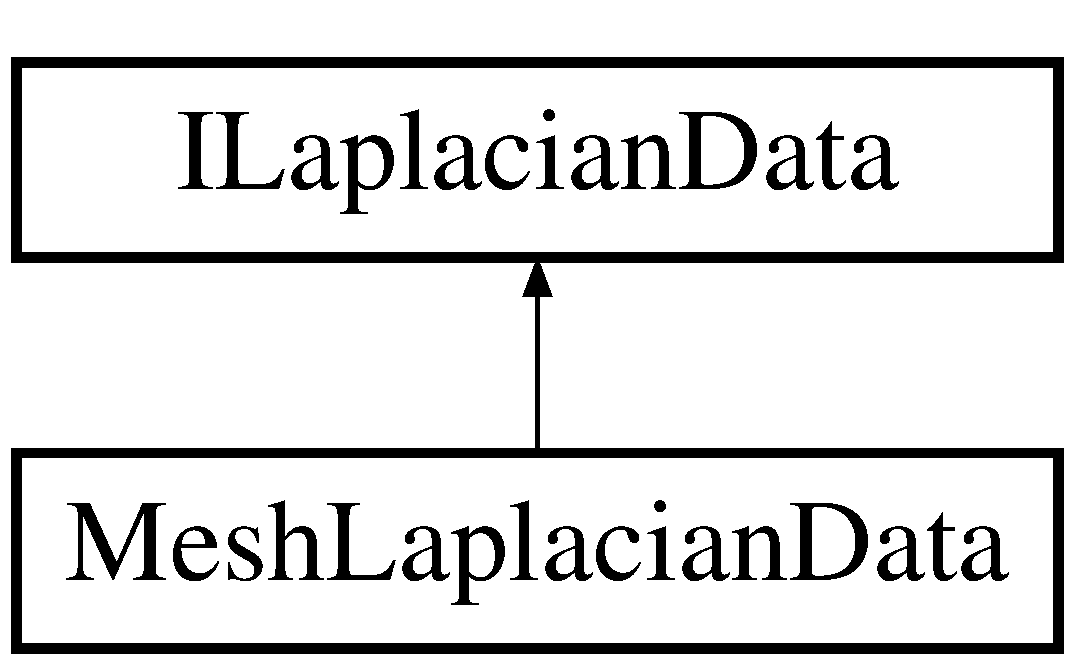
\includegraphics[height=2.000000cm]{class_mesh_laplacian_data}
\end{center}
\end{figure}
\subsection*{Public Member Functions}
\begin{DoxyCompactItemize}
\item 
\hyperlink{class_mesh_laplacian_data_a5f57380117063fed3c758070836deed8}{Mesh\+Laplacian\+Data} (const M\+Dag\+Path \&geometry\+Path)
\item 
\hyperlink{class_mesh_laplacian_data_a0baa5e645b1f92cbd77094d9e8fe371b}{Mesh\+Laplacian\+Data} (const M\+Object \&geometry\+Object)
\item 
\hypertarget{class_mesh_laplacian_data_a226a9e35ed02adcc11ea372bdaa5da1a}{virtual \hyperlink{class_mesh_laplacian_data_a226a9e35ed02adcc11ea372bdaa5da1a}{$\sim$\+Mesh\+Laplacian\+Data} ()}\label{class_mesh_laplacian_data_a226a9e35ed02adcc11ea372bdaa5da1a}

\begin{DoxyCompactList}\small\item\em Destructor. \end{DoxyCompactList}\item 
const Eigen\+::\+Sparse\+Matrix$<$ double $>$ \hyperlink{class_mesh_laplacian_data_a9efe80838593c46fac7baa77ef506559}{Get\+Laplacian\+Matrix} (int num\+Functions=3)
\begin{DoxyCompactList}\small\item\em Get Laplacian data. \end{DoxyCompactList}\end{DoxyCompactItemize}
\subsection*{Additional Inherited Members}


\subsection{Detailed Description}
Laplacian data. 

\subsection{Constructor \& Destructor Documentation}
\hypertarget{class_mesh_laplacian_data_a5f57380117063fed3c758070836deed8}{\index{Mesh\+Laplacian\+Data@{Mesh\+Laplacian\+Data}!Mesh\+Laplacian\+Data@{Mesh\+Laplacian\+Data}}
\index{Mesh\+Laplacian\+Data@{Mesh\+Laplacian\+Data}!Mesh\+Laplacian\+Data@{Mesh\+Laplacian\+Data}}
\subsubsection[{Mesh\+Laplacian\+Data}]{\setlength{\rightskip}{0pt plus 5cm}Mesh\+Laplacian\+Data\+::\+Mesh\+Laplacian\+Data (
\begin{DoxyParamCaption}
\item[{const M\+Dag\+Path \&}]{geometry\+Path}
\end{DoxyParamCaption}
)}}\label{class_mesh_laplacian_data_a5f57380117063fed3c758070836deed8}

\begin{DoxyParams}{Parameters}
{\em geometry\+Path} & target geometry dag path \\
\hline
\end{DoxyParams}
\hypertarget{class_mesh_laplacian_data_a0baa5e645b1f92cbd77094d9e8fe371b}{\index{Mesh\+Laplacian\+Data@{Mesh\+Laplacian\+Data}!Mesh\+Laplacian\+Data@{Mesh\+Laplacian\+Data}}
\index{Mesh\+Laplacian\+Data@{Mesh\+Laplacian\+Data}!Mesh\+Laplacian\+Data@{Mesh\+Laplacian\+Data}}
\subsubsection[{Mesh\+Laplacian\+Data}]{\setlength{\rightskip}{0pt plus 5cm}Mesh\+Laplacian\+Data\+::\+Mesh\+Laplacian\+Data (
\begin{DoxyParamCaption}
\item[{const M\+Object \&}]{geometry\+Object}
\end{DoxyParamCaption}
)}}\label{class_mesh_laplacian_data_a0baa5e645b1f92cbd77094d9e8fe371b}

\begin{DoxyParams}{Parameters}
{\em geometry\+Object} & target geometry object \\
\hline
\end{DoxyParams}


\subsection{Member Function Documentation}
\hypertarget{class_mesh_laplacian_data_a9efe80838593c46fac7baa77ef506559}{\index{Mesh\+Laplacian\+Data@{Mesh\+Laplacian\+Data}!Get\+Laplacian\+Matrix@{Get\+Laplacian\+Matrix}}
\index{Get\+Laplacian\+Matrix@{Get\+Laplacian\+Matrix}!Mesh\+Laplacian\+Data@{Mesh\+Laplacian\+Data}}
\subsubsection[{Get\+Laplacian\+Matrix}]{\setlength{\rightskip}{0pt plus 5cm}const Eigen\+::\+Sparse\+Matrix$<$ double $>$ Mesh\+Laplacian\+Data\+::\+Get\+Laplacian\+Matrix (
\begin{DoxyParamCaption}
\item[{int}]{num\+Functions = {\ttfamily 3}}
\end{DoxyParamCaption}
)\hspace{0.3cm}{\ttfamily [virtual]}}}\label{class_mesh_laplacian_data_a9efe80838593c46fac7baa77ef506559}


Get Laplacian data. 


\begin{DoxyParams}{Parameters}
{\em num\+Functions} & the number of functions (e.\+g. 3 for point xyz.) \\
\hline
\end{DoxyParams}
\begin{DoxyReturn}{Returns}
Laplacian\+Matrix output Laplacian matrix data. Eigen\+::\+Sparse\+Matrix$<$double$>$ type. 
\end{DoxyReturn}


Implements \hyperlink{class_i_laplacian_data_ae5d1999d7e077fae5e415ce811d71dba}{I\+Laplacian\+Data}.



The documentation for this class was generated from the following files\+:\begin{DoxyCompactItemize}
\item 
C\+:/\+Users/tody/\+Documents/\+Git\+Hub/\+Maya\+Plugin\+Samples/\+Laplacian\+Smoother/src/Mesh\+Laplacian\+Data.\+h\item 
C\+:/\+Users/tody/\+Documents/\+Git\+Hub/\+Maya\+Plugin\+Samples/\+Laplacian\+Smoother/src/Mesh\+Laplacian\+Data.\+cpp\end{DoxyCompactItemize}

\hypertarget{class_time_counter}{\section{Time\+Counter Class Reference}
\label{class_time_counter}\index{Time\+Counter@{Time\+Counter}}
}


\hyperlink{class_time_counter}{Time\+Counter} implementation.  




{\ttfamily \#include $<$Time\+Counter.\+h$>$}

\subsection*{Public Member Functions}
\begin{DoxyCompactItemize}
\item 
\hypertarget{class_time_counter_a97c725f083ddea9e113b2af85d564995}{\hyperlink{class_time_counter_a97c725f083ddea9e113b2af85d564995}{Time\+Counter} (const std\+::string \&name)}\label{class_time_counter_a97c725f083ddea9e113b2af85d564995}

\begin{DoxyCompactList}\small\item\em Constructor. \end{DoxyCompactList}\item 
\hypertarget{class_time_counter_a29b72a1f27b48bda15e15dae2ce98a51}{virtual \hyperlink{class_time_counter_a29b72a1f27b48bda15e15dae2ce98a51}{$\sim$\+Time\+Counter} ()}\label{class_time_counter_a29b72a1f27b48bda15e15dae2ce98a51}

\begin{DoxyCompactList}\small\item\em Destructor. \end{DoxyCompactList}\item 
\hypertarget{class_time_counter_a32cb7d643afd5c748549900417a8eb60}{void \hyperlink{class_time_counter_a32cb7d643afd5c748549900417a8eb60}{set\+Name} (const std\+::string \&name)}\label{class_time_counter_a32cb7d643afd5c748549900417a8eb60}

\begin{DoxyCompactList}\small\item\em Set the name of the counter. \end{DoxyCompactList}\item 
\hypertarget{class_time_counter_acf8d1fd02676e6d8e3f44ceef8fce188}{const std\+::string \& \hyperlink{class_time_counter_acf8d1fd02676e6d8e3f44ceef8fce188}{get\+Name} () const }\label{class_time_counter_acf8d1fd02676e6d8e3f44ceef8fce188}

\begin{DoxyCompactList}\small\item\em Return the name of the counter. \end{DoxyCompactList}\item 
\hypertarget{class_time_counter_a27d1998986d33b4d037b7ed21f121b97}{double \hyperlink{class_time_counter_a27d1998986d33b4d037b7ed21f121b97}{get\+Elapsed\+Time} ()}\label{class_time_counter_a27d1998986d33b4d037b7ed21f121b97}

\begin{DoxyCompactList}\small\item\em Get elapsed time. \end{DoxyCompactList}\item 
\hypertarget{class_time_counter_a08647c9c74e1b6ba366df28e1d27e67e}{bool \hyperlink{class_time_counter_a08647c9c74e1b6ba366df28e1d27e67e}{is\+Running} ()}\label{class_time_counter_a08647c9c74e1b6ba366df28e1d27e67e}

\begin{DoxyCompactList}\small\item\em Return if the counter is running or not. \end{DoxyCompactList}\item 
\hypertarget{class_time_counter_aa10a840834e2d49c3979f448212a59de}{void \hyperlink{class_time_counter_aa10a840834e2d49c3979f448212a59de}{start} ()}\label{class_time_counter_aa10a840834e2d49c3979f448212a59de}

\begin{DoxyCompactList}\small\item\em Start the counter. \end{DoxyCompactList}\item 
\hypertarget{class_time_counter_a2f5bc943c35f19ccad8ef12cf7876d57}{double \hyperlink{class_time_counter_a2f5bc943c35f19ccad8ef12cf7876d57}{pause} ()}\label{class_time_counter_a2f5bc943c35f19ccad8ef12cf7876d57}

\begin{DoxyCompactList}\small\item\em Stop without reseting. \end{DoxyCompactList}\item 
double \hyperlink{class_time_counter_a7ab5f9bdfef98289f3013b3a8c250925}{reset} ()
\begin{DoxyCompactList}\small\item\em Rest the counter. \end{DoxyCompactList}\end{DoxyCompactItemize}
\subsection*{Friends}
\begin{DoxyCompactItemize}
\item 
std\+::ostream \& \hyperlink{class_time_counter_a0b9687b6bb68ac0433cb13f912e236cf}{operator$<$$<$} (std\+::ostream \&out, \hyperlink{class_time_counter}{Time\+Counter} \&counter)
\begin{DoxyCompactList}\small\item\em Output string for the counter. \end{DoxyCompactList}\end{DoxyCompactItemize}


\subsection{Detailed Description}
\hyperlink{class_time_counter}{Time\+Counter} implementation. 

\subsection{Member Function Documentation}
\hypertarget{class_time_counter_a7ab5f9bdfef98289f3013b3a8c250925}{\index{Time\+Counter@{Time\+Counter}!reset@{reset}}
\index{reset@{reset}!Time\+Counter@{Time\+Counter}}
\subsubsection[{reset}]{\setlength{\rightskip}{0pt plus 5cm}double Time\+Counter\+::reset (
\begin{DoxyParamCaption}
{}
\end{DoxyParamCaption}
)}}\label{class_time_counter_a7ab5f9bdfef98289f3013b3a8c250925}


Rest the counter. 

\begin{DoxyReturn}{Returns}
elapsed time before reset. 
\end{DoxyReturn}


\subsection{Friends And Related Function Documentation}
\hypertarget{class_time_counter_a0b9687b6bb68ac0433cb13f912e236cf}{\index{Time\+Counter@{Time\+Counter}!operator$<$$<$@{operator$<$$<$}}
\index{operator$<$$<$@{operator$<$$<$}!Time\+Counter@{Time\+Counter}}
\subsubsection[{operator$<$$<$}]{\setlength{\rightskip}{0pt plus 5cm}std\+::ostream\& operator$<$$<$ (
\begin{DoxyParamCaption}
\item[{std\+::ostream \&}]{out, }
\item[{{\bf Time\+Counter} \&}]{counter}
\end{DoxyParamCaption}
)\hspace{0.3cm}{\ttfamily [friend]}}}\label{class_time_counter_a0b9687b6bb68ac0433cb13f912e236cf}


Output string for the counter. 

Output will be \char`\"{}name\+: ...\mbox{[}sec\mbox{]}\char`\"{} 

The documentation for this class was generated from the following files\+:\begin{DoxyCompactItemize}
\item 
C\+:/\+Users/tody/\+Documents/\+Git\+Hub/\+Maya\+Plugin\+Samples/\+Laplacian\+Smoother/src/\hyperlink{_time_counter_8h}{Time\+Counter.\+h}\item 
C\+:/\+Users/tody/\+Documents/\+Git\+Hub/\+Maya\+Plugin\+Samples/\+Laplacian\+Smoother/src/Time\+Counter.\+cpp\end{DoxyCompactItemize}

\chapter{File Documentation}
\hypertarget{_init_plugin_8cpp}{\section{C\+:/\+Users/tody/\+Documents/\+Git\+Hub/\+Maya\+Plugin\+Samples/\+Laplacian\+Smoother/src/\+Init\+Plugin.cpp File Reference}
\label{_init_plugin_8cpp}\index{C\+:/\+Users/tody/\+Documents/\+Git\+Hub/\+Maya\+Plugin\+Samples/\+Laplacian\+Smoother/src/\+Init\+Plugin.\+cpp@{C\+:/\+Users/tody/\+Documents/\+Git\+Hub/\+Maya\+Plugin\+Samples/\+Laplacian\+Smoother/src/\+Init\+Plugin.\+cpp}}
}


Plugin functions for \hyperlink{class_laplacian_smoother}{Laplacian\+Smoother}.  


{\ttfamily \#include $<$maya/\+M\+Fn\+Plugin.\+h$>$}\\*
{\ttfamily \#include \char`\"{}Laplacian\+Smoother.\+h\char`\"{}}\\*
\subsection*{Functions}
\begin{DoxyCompactItemize}
\item 
\hypertarget{_init_plugin_8cpp_a0210a4502206b305079c736839c98c70}{M\+Status \hyperlink{_init_plugin_8cpp_a0210a4502206b305079c736839c98c70}{initialize\+Plugin} (M\+Object obj)}\label{_init_plugin_8cpp_a0210a4502206b305079c736839c98c70}

\begin{DoxyCompactList}\small\item\em Initialize plugin for \hyperlink{class_laplacian_smoother}{Laplacian\+Smoother}. \end{DoxyCompactList}\item 
\hypertarget{_init_plugin_8cpp_a91038a1d4238b2c1af6a8f40fc83c278}{M\+Status \hyperlink{_init_plugin_8cpp_a91038a1d4238b2c1af6a8f40fc83c278}{uninitialize\+Plugin} (M\+Object obj)}\label{_init_plugin_8cpp_a91038a1d4238b2c1af6a8f40fc83c278}

\begin{DoxyCompactList}\small\item\em Uninitialize plugin for \hyperlink{class_laplacian_smoother}{Laplacian\+Smoother}. \end{DoxyCompactList}\end{DoxyCompactItemize}


\subsection{Detailed Description}
Plugin functions for \hyperlink{class_laplacian_smoother}{Laplacian\+Smoother}. 

\begin{DoxyAuthor}{Author}
Tody 
\end{DoxyAuthor}
\begin{DoxyDate}{Date}
2015/03/17 
\end{DoxyDate}

\hypertarget{_laplacian_smoother_8cpp}{\section{C\+:/\+Users/tody/\+Documents/\+Git\+Hub/\+Maya\+Plugin\+Samples/\+Laplacian\+Smoother/src/\+Laplacian\+Smoother.cpp File Reference}
\label{_laplacian_smoother_8cpp}\index{C\+:/\+Users/tody/\+Documents/\+Git\+Hub/\+Maya\+Plugin\+Samples/\+Laplacian\+Smoother/src/\+Laplacian\+Smoother.\+cpp@{C\+:/\+Users/tody/\+Documents/\+Git\+Hub/\+Maya\+Plugin\+Samples/\+Laplacian\+Smoother/src/\+Laplacian\+Smoother.\+cpp}}
}


\hyperlink{class_laplacian_smoother}{Laplacian\+Smoother} definition.  


{\ttfamily \#include \char`\"{}Laplacian\+Smoother.\+h\char`\"{}}\\*
{\ttfamily \#include $<$maya/\+M\+Fn\+Numeric\+Attribute.\+h$>$}\\*
{\ttfamily \#include $<$maya/\+M\+Data\+Handle.\+h$>$}\\*
{\ttfamily \#include $<$Eigen/\+Dense$>$}\\*
{\ttfamily \#include $<$Eigen/\+Sparse$>$}\\*
{\ttfamily \#include $<$Eigen/\+Sparse\+L\+U$>$}\\*
{\ttfamily \#include \char`\"{}Mesh\+Laplacian\+Data.\+h\char`\"{}}\\*
{\ttfamily \#include \char`\"{}Maya\+Eigen.\+h\char`\"{}}\\*
{\ttfamily \#include \char`\"{}Time\+Counter.\+h\char`\"{}}\\*
\subsection*{Macros}
\begin{DoxyCompactItemize}
\item 
\hypertarget{_laplacian_smoother_8cpp_aa93624b0b2836d2510e8c92ae951d817}{\#define {\bfseries E\+I\+G\+E\+N\+\_\+\+Y\+E\+S\+\_\+\+I\+\_\+\+K\+N\+O\+W\+\_\+\+S\+P\+A\+R\+S\+E\+\_\+\+M\+O\+D\+U\+L\+E\+\_\+\+I\+S\+\_\+\+N\+O\+T\+\_\+\+S\+T\+A\+B\+L\+E\+\_\+\+Y\+E\+T}}\label{_laplacian_smoother_8cpp_aa93624b0b2836d2510e8c92ae951d817}

\item 
\#define \hyperlink{_laplacian_smoother_8cpp_a6b9ddb1ef0cccc80937d6e35820b65fe}{M\+A\+K\+E\+\_\+\+I\+N\+P\+U\+T}(attr)
\begin{DoxyCompactList}\small\item\em Macro for an input attribute. \end{DoxyCompactList}\item 
\#define \hyperlink{_laplacian_smoother_8cpp_ac97edf1facf2243bc31852a0d1332d87}{M\+A\+K\+E\+\_\+\+O\+U\+T\+P\+U\+T}(attr)
\begin{DoxyCompactList}\small\item\em Macro for an output attribute. \end{DoxyCompactList}\end{DoxyCompactItemize}


\subsection{Detailed Description}
\hyperlink{class_laplacian_smoother}{Laplacian\+Smoother} definition. 

\begin{DoxyAuthor}{Author}
Tody
\end{DoxyAuthor}
date 2014/07/06 

\subsection{Macro Definition Documentation}
\hypertarget{_laplacian_smoother_8cpp_a6b9ddb1ef0cccc80937d6e35820b65fe}{\index{Laplacian\+Smoother.\+cpp@{Laplacian\+Smoother.\+cpp}!M\+A\+K\+E\+\_\+\+I\+N\+P\+U\+T@{M\+A\+K\+E\+\_\+\+I\+N\+P\+U\+T}}
\index{M\+A\+K\+E\+\_\+\+I\+N\+P\+U\+T@{M\+A\+K\+E\+\_\+\+I\+N\+P\+U\+T}!Laplacian\+Smoother.\+cpp@{Laplacian\+Smoother.\+cpp}}
\subsubsection[{M\+A\+K\+E\+\_\+\+I\+N\+P\+U\+T}]{\setlength{\rightskip}{0pt plus 5cm}\#define M\+A\+K\+E\+\_\+\+I\+N\+P\+U\+T(
\begin{DoxyParamCaption}
\item[{}]{attr}
\end{DoxyParamCaption}
)}}\label{_laplacian_smoother_8cpp_a6b9ddb1ef0cccc80937d6e35820b65fe}
{\bfseries Value\+:}
\begin{DoxyCode}
CHECK\_MSTATUS(attr.setKeyable(\textcolor{keyword}{true})); \(\backslash\)
    CHECK\_MSTATUS(attr.setStorable(\textcolor{keyword}{true})); \(\backslash\)
    CHECK\_MSTATUS(attr.setReadable(\textcolor{keyword}{true})); \(\backslash\)
    CHECK\_MSTATUS(attr.setWritable(\textcolor{keyword}{true}));
\end{DoxyCode}


Macro for an input attribute. 

\hypertarget{_laplacian_smoother_8cpp_ac97edf1facf2243bc31852a0d1332d87}{\index{Laplacian\+Smoother.\+cpp@{Laplacian\+Smoother.\+cpp}!M\+A\+K\+E\+\_\+\+O\+U\+T\+P\+U\+T@{M\+A\+K\+E\+\_\+\+O\+U\+T\+P\+U\+T}}
\index{M\+A\+K\+E\+\_\+\+O\+U\+T\+P\+U\+T@{M\+A\+K\+E\+\_\+\+O\+U\+T\+P\+U\+T}!Laplacian\+Smoother.\+cpp@{Laplacian\+Smoother.\+cpp}}
\subsubsection[{M\+A\+K\+E\+\_\+\+O\+U\+T\+P\+U\+T}]{\setlength{\rightskip}{0pt plus 5cm}\#define M\+A\+K\+E\+\_\+\+O\+U\+T\+P\+U\+T(
\begin{DoxyParamCaption}
\item[{}]{attr}
\end{DoxyParamCaption}
)}}\label{_laplacian_smoother_8cpp_ac97edf1facf2243bc31852a0d1332d87}
{\bfseries Value\+:}
\begin{DoxyCode}
CHECK\_MSTATUS(attr.setKeyable(\textcolor{keyword}{false})); \(\backslash\)
    CHECK\_MSTATUS(attr.setStorable(\textcolor{keyword}{true})); \(\backslash\)
    CHECK\_MSTATUS(attr.setReadable(\textcolor{keyword}{true})); \(\backslash\)
    CHECK\_MSTATUS(attr.setWritable(\textcolor{keyword}{true}));
\end{DoxyCode}


Macro for an output attribute. 


\hypertarget{_laplacian_smoother_8h}{\section{C\+:/\+Users/tody/\+Documents/\+Git\+Hub/\+Maya\+Plugin\+Samples/\+Laplacian\+Smoother/src/\+Laplacian\+Smoother.h File Reference}
\label{_laplacian_smoother_8h}\index{C\+:/\+Users/tody/\+Documents/\+Git\+Hub/\+Maya\+Plugin\+Samples/\+Laplacian\+Smoother/src/\+Laplacian\+Smoother.\+h@{C\+:/\+Users/tody/\+Documents/\+Git\+Hub/\+Maya\+Plugin\+Samples/\+Laplacian\+Smoother/src/\+Laplacian\+Smoother.\+h}}
}
{\ttfamily \#include $<$maya/\+M\+Px\+Deformer\+Node.\+h$>$}\\*
{\ttfamily \#include $<$Eigen/\+Sparse$>$}\\*
\subsection*{Classes}
\begin{DoxyCompactItemize}
\item 
class \hyperlink{class_laplacian_smoother}{Laplacian\+Smoother}
\begin{DoxyCompactList}\small\item\em \hyperlink{class_laplacian_smoother}{Laplacian\+Smoother} implementation. \end{DoxyCompactList}\end{DoxyCompactItemize}


\subsection{Detailed Description}
\begin{DoxyAuthor}{Author}
Tody \hyperlink{class_laplacian_smoother}{Laplacian\+Smoother} definition. 
\end{DoxyAuthor}
\begin{DoxyDate}{Date}
2015/03/17 
\end{DoxyDate}

\hypertarget{_maya_eigen_8cpp}{\section{C\+:/\+Users/tody/\+Documents/\+Git\+Hub/\+Maya\+Plugin\+Samples/\+Laplacian\+Smoother/src/\+Maya\+Eigen.cpp File Reference}
\label{_maya_eigen_8cpp}\index{C\+:/\+Users/tody/\+Documents/\+Git\+Hub/\+Maya\+Plugin\+Samples/\+Laplacian\+Smoother/src/\+Maya\+Eigen.\+cpp@{C\+:/\+Users/tody/\+Documents/\+Git\+Hub/\+Maya\+Plugin\+Samples/\+Laplacian\+Smoother/src/\+Maya\+Eigen.\+cpp}}
}


\hyperlink{class_laplacian_smoother}{Laplacian\+Smoother} definition.  


{\ttfamily \#include \char`\"{}Maya\+Eigen.\+h\char`\"{}}\\*
{\ttfamily \#include $<$maya/\+M\+Fn\+Mesh.\+h$>$}\\*
{\ttfamily \#include $<$maya/\+M\+Point\+Array.\+h$>$}\\*
{\ttfamily \#include $<$maya/\+M\+Float\+Vector\+Array.\+h$>$}\\*


\subsection{Detailed Description}
\hyperlink{class_laplacian_smoother}{Laplacian\+Smoother} definition. 

\begin{DoxyAuthor}{Author}
Tody \hyperlink{class_maya_eigen}{Maya\+Eigen} definition. date 2015/03/17 
\end{DoxyAuthor}

\hypertarget{_maya_eigen_8h}{\section{C\+:/\+Users/tody/\+Documents/\+Git\+Hub/\+Maya\+Plugin\+Samples/\+Laplacian\+Smoother/src/\+Maya\+Eigen.h File Reference}
\label{_maya_eigen_8h}\index{C\+:/\+Users/tody/\+Documents/\+Git\+Hub/\+Maya\+Plugin\+Samples/\+Laplacian\+Smoother/src/\+Maya\+Eigen.\+h@{C\+:/\+Users/tody/\+Documents/\+Git\+Hub/\+Maya\+Plugin\+Samples/\+Laplacian\+Smoother/src/\+Maya\+Eigen.\+h}}
}
{\ttfamily \#include $<$maya/\+M\+Object.\+h$>$}\\*
{\ttfamily \#include $<$Eigen/\+Sparse$>$}\\*
\subsection*{Classes}
\begin{DoxyCompactItemize}
\item 
class \hyperlink{class_maya_eigen}{Maya\+Eigen}
\begin{DoxyCompactList}\small\item\em \hyperlink{class_maya_eigen}{Maya\+Eigen} implementation. \end{DoxyCompactList}\end{DoxyCompactItemize}


\subsection{Detailed Description}
\begin{DoxyAuthor}{Author}
Tody \hyperlink{class_maya_eigen}{Maya\+Eigen} definition. 
\end{DoxyAuthor}
\begin{DoxyDate}{Date}
2015/03/17 
\end{DoxyDate}

\hypertarget{_time_counter_8h}{\section{C\+:/\+Users/tody/\+Documents/\+Git\+Hub/\+Maya\+Plugin\+Samples/\+Laplacian\+Smoother/src/\+Time\+Counter.h File Reference}
\label{_time_counter_8h}\index{C\+:/\+Users/tody/\+Documents/\+Git\+Hub/\+Maya\+Plugin\+Samples/\+Laplacian\+Smoother/src/\+Time\+Counter.\+h@{C\+:/\+Users/tody/\+Documents/\+Git\+Hub/\+Maya\+Plugin\+Samples/\+Laplacian\+Smoother/src/\+Time\+Counter.\+h}}
}


\hyperlink{class_time_counter}{Time\+Counter} class definition.  


{\ttfamily \#include $<$time.\+h$>$}\\*
{\ttfamily \#include $<$ostream$>$}\\*
{\ttfamily \#include $<$string$>$}\\*
\subsection*{Classes}
\begin{DoxyCompactItemize}
\item 
class \hyperlink{class_time_counter}{Time\+Counter}
\begin{DoxyCompactList}\small\item\em \hyperlink{class_time_counter}{Time\+Counter} implementation. \end{DoxyCompactList}\end{DoxyCompactItemize}


\subsection{Detailed Description}
\hyperlink{class_time_counter}{Time\+Counter} class definition. 

\begin{DoxyAuthor}{Author}
Tody 
\end{DoxyAuthor}
\begin{DoxyDate}{Date}

\end{DoxyDate}

%--- End generated contents ---

% Index
\newpage
\phantomsection
\addcontentsline{toc}{chapter}{Index}
\printindex

\end{document}
